% id: 0211
% book: RPM 중3-2 수학 · 02 삼각비의 활용
% section: 유형 11 평행사변형의 넓이
% figure: crop:fig-0211.png
% answer: ③
% answer_source: 답지
% variant_level: 0 (원본 전사)
% 이 파일은 build.mjs 가 items.json 에서 만든다. 고칠 때는 items.json 을 고친다.
\smash{\raisebox{4.5mm}{\dmkichul{대표문제}}}
\noindent\begin{minipage}[t]{0.58\linewidth}\vspace{0pt}\raggedright 오른쪽 그림과 같은 마름모~$\pt{ABCD}$의 넓이가 $18\sqrt{2}\mkern3mu \mathrm{cm}^2$일 때, 마름모~$\pt{ABCD}$의 한 변의 길이는?\end{minipage}\hfill\begin{minipage}[t]{0.4\linewidth}\vspace{0pt}\centering \setlength{\dmfigw}{96.5pt}\ifdim\dmfigw>\linewidth\setlength{\dmfigw}{\linewidth}\fi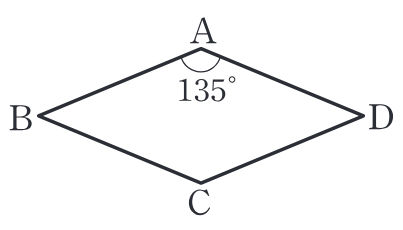
\includegraphics[width=\dmfigw]{figures/fig-0211.png}\end{minipage}\par
\begin{choices32}{$4\mkern3mu \mathrm{cm}$}{$5\mkern3mu \mathrm{cm}$}{$6\mkern3mu \mathrm{cm}$}{$7\mkern3mu \mathrm{cm}$}{$8\mkern3mu \mathrm{cm}$}\end{choices32}
